\documentclass{beamer}

\usepackage{beamerthemesplit}
\usepackage{graphicx}
\usepackage{color, natbib, hyperref}
\usepackage{bibentry}
\usepackage[export]{adjustbox}% http://ctan.org/pkg/adjustbox
\usepackage{multicol}
\usepackage{tikz}

\nobibliography*

% define colors
\definecolor{jblue}  {RGB}{20,50,100}
\definecolor{ngreen} {RGB}{98,158,31}

%theme

\usetheme{boxes} 
%\usecolortheme{seahorse} 
\setbeamertemplate{items}[default] 
%\setbeamercovered{transparent}
\setbeamertemplate{blocks}[rounded]
\setbeamertemplate{navigation symbols}{} 
% set the basic colors
\setbeamercolor{palette primary}   {fg=black,bg=white}
\setbeamercolor{palette secondary} {fg=black,bg=white}
\setbeamercolor{palette tertiary}  {bg=jblue,fg=white}
\setbeamercolor{palette quaternary}{fg=black,bg=white}
\setbeamercolor{structure}{fg=jblue}
\setbeamercolor{titlelike}{bg=jblue,fg=white}
\setbeamercolor{frametitle}{bg=jblue!10,fg=jblue}
\setbeamercolor{cboxb}{fg=black,bg=jblue}
\setbeamercolor{cboxr}{fg=black,bg=red}

% reduce space before/after equations
\expandafter\def\expandafter\normalsize\expandafter{%
    \normalsize
    \setlength\abovedisplayskip{1pt}
    \setlength\belowdisplayskip{1pt}
    \setlength\abovedisplayshortskip{1pt}
    \setlength\belowdisplayshortskip{1pt}
}

% set colors for itemize/enumerate
\setbeamercolor{item}{fg=ngreen}
\setbeamercolor{item projected}{fg=white,bg=ngreen}

% set colors for blocks
\setbeamercolor{block title}{fg=ngreen,bg=white}
\setbeamercolor{block body}{fg=black,bg=jblue!10}

% set colors for alerted blocks (blocks with frame)
\setbeamercolor{block alerted title}{fg=white,bg=jblue}
\setbeamercolor{block alerted body}{fg=black,bg=jblue!10}
\setbeamercolor{block alerted title}{fg=white,bg=dblue!70} % Colors of the highlighted block titles
\setbeamercolor{block alerted body}{fg=black,bg=dblue!10} % Colors of the body of highlighted blocks

% set the fonts
\usefonttheme{professionalfonts}

\setbeamerfont{section in head/foot}{series=\bfseries}
\setbeamerfont{block title}{series=\bfseries}
\setbeamerfont{block alerted title}{series=\bfseries}
\setbeamerfont{frametitle}{series=\bfseries}
\setbeamerfont{frametitle}{size=\Large}
\setbeamerfont{block body}{series=\mdseries}
\setbeamerfont{caption}{series=\mdseries}
\setbeamerfont{headline}{series=\mdseries}


% set some beamer theme options
\setbeamertemplate{title page}[default][colsep=-4bp,rounded=true]
\setbeamertemplate{sections/subsections in toc}[square]
\setbeamertemplate{items}[circle]
\setbeamertemplate{blocks}[width=0.0]
\beamertemplatenavigationsymbolsempty

% Custom colors
\usepackage{color}
%\definecolor{deepblue}{rgb}{0,0,0.5}
%\definecolor{deepred}{rgb}{0.6,0,0}
%\definecolor{deepgreen}{rgb}{0,0.5,0}
\definecolor{Code}{rgb}{0,0,0}
\definecolor{Decorators}{rgb}{0.5,0.5,0.5}
\definecolor{Numbers}{rgb}{0.5,0,0}
\definecolor{MatchingBrackets}{rgb}{0.25,0.5,0.5}
\definecolor{Strings}{rgb}{0.75,0,0}
\definecolor{self}{rgb}{0,0,0}
\definecolor{Keywords}{rgb}{0,0.63,0}
\definecolor{Comments}{rgb}{0,0.63,1}
\definecolor{Backquotes}{rgb}{0,0,0}
\definecolor{Classname}{rgb}{0,0,0}
\definecolor{FunctionName}{rgb}{0,0,0}
\definecolor{Operators}{rgb}{0,0,0}

% Default fixed font does not support bold face
\usepackage[utf8]{inputenc}
\DeclareFixedFont{\ttb}{T1}{txtt}{bx}{n}{12} % for bold
\DeclareFixedFont{\ttm}{T1}{txtt}{m}{n}{12}  % for normal

% Python style for highlighting
\usepackage{listings}
\newcommand\rstyle{\lstset{
language=R,
%numbers=left,
%numberstyle=\footnotesize,
%numbersep=1em,
%xleftmargin=1em,
framextopmargin=0em,
framexbottommargin=0em,
showspaces=false,
showtabs=false,
showstringspaces=false,
frame=l,
tabsize=4,
% Basic
basicstyle=\ttfamily\scriptsize,
otherkeywords={!,!=,~,$,*,\&,\%/\%,\%*\%,\%\%,<-,<<-},
%keywordstyle={\color{Keywords}\bfseries},
% Comments
commentstyle=\color{Comments}\slshape,
%% Strings
stringstyle=\color{Strings},
morecomment=[s][\color{Strings}]{"""}{"""},
morecomment=[s][\color{Strings}]{'''}{'''},
% keywords
morekeywords={},
keywordstyle={\color{Keywords}\bfseries},
deletekeywords={ts, mat, time, sample, response, stat},
% additional keywords
morekeywords={[2]@response, group, stratum, stat},
keywordstyle={[2]\color{Decorators}\slshape},
emph={self},
emphstyle={\color{self}\slshape},
frame=tb,                         % Any extra options here
showstringspaces=false            % 
}}

% R environment
\lstnewenvironment{rcode}[1][]
{
\rstyle
\lstset{#1}
}
{}


% R for inline
\newcommand\rinline[1]{{\rstyle\lstinline!#1!}}



% Math macros
\newcommand{\cD}{{\mathcal D}}
\newcommand{\cF}{{\mathcal F}}
\newcommand{\todo}[1]{{\color{red}{TO DO: \sc #1}}}

\newcommand{\reals}{\mathbb{R}}
\newcommand{\integers}{\mathbb{Z}}
\newcommand{\naturals}{\mathbb{N}}
\newcommand{\rationals}{\mathbb{Q}}

\newcommand{\ind}[1]{1_{#1}} % Indicator function
\newcommand{\pr}{\mathbb{P}} % Generic probability
\newcommand{\ex}{\mathbb{E}} % Generic expectation
\newcommand{\var}{\textrm{Var}}
\newcommand{\cov}{\textrm{Cov}}

\newcommand{\normal}{N} % for normal distribution (can probably skip this)
\newcommand{\eps}{\varepsilon}
\newcommand\independent{\protect\mathpalette{\protect\independenT}{\perp}}
\def\independenT#1#2{\mathrel{\rlap{$#1#2$}\mkern2mu{#1#2}}}

\newcommand{\convd}{\stackrel{d}{\longrightarrow}} % convergence in distribution/law/measure
\newcommand{\convp}{\stackrel{P}{\longrightarrow}} % convergence in probability
\newcommand{\convas}{\stackrel{\textrm{a.s.}}{\longrightarrow}} % convergence almost surely

\newcommand{\eqd}{\stackrel{d}{=}} % equal in distribution/law/measure
\newcommand{\argmax}{\arg\!\max}
\newcommand{\argmin}{\arg\!\min}


\mode<presentation>

\title[permute]{permuter: An R Package for Randomization Inference}
\author{\Large Kellie Ottoboni}
\institute[]{Department of Statistics, UC Berkeley\\Berkeley Institute for Data Science}
\date{June 28, 2016\\\small useR! Stanford}

\begin{document}

\frame{
\titlepage
\vfill
\begin{columns}[T]
\begin{column}{.5\textwidth}
\begin{center}
\vspace{25pt}

\includegraphics[width=\textwidth]{fig/logo/dept1.pdf}
\end{center}
\end{column}
\begin{column}{.3\textwidth}
\end{column}
\begin{column}{.3\textwidth}
\begin{center}

\includegraphics[width=0.9\textwidth]{fig/logo/BIDS.png}
\end{center}
\end{column}
\end{columns}
}

\AtBeginSection[]
{
   \begin{frame}
       \frametitle{Outline}
       \tableofcontents[currentsection]
   \end{frame}
}



\section[Introduction]{Introduction}


\frame{
\frametitle{Permutation tests}

\begin{itemize}
\itemsep15pt
\item \citet{fisher_design_1935} introduced permutation tests for randomized experiments
\item Rely on assumptions about randomization or exchangeability, rather than parametric assumptions, IID sampling, etc.
\end{itemize}
\vspace{20pt}
\begin{block}{James \citet{bradley1968distribution}}
``[a] corresponding parametric test is valid only to the extent that it results in the same statistical decision [as the randomization test].'' 
\end{block}

}


\frame{
\frametitle{Permutation tests}

R has several packages for randomization inference.
\begin{multicols}{2}
\begin{itemize}
\item \texttt{ri} %by Peter Aronow and Cyrus Samii

{\tiny\textit{``This package provides a set of tools for conducting exact or approximate inference for randomized experiments of arbitrary design. The primary functionality of the package is in the generation, manipulation and use of permutation matrices implied by given experimental designs...''}\par}
\item \texttt{RItools} %by Mark Fredrickson

{\tiny\textit{``The RItools package implements useful functions for implementing randomization inference based statistical tests. The package provides tools for testing balance of observed covariates in observational studies using the methodology of:...The package also provides outcome analysis of simple or block randomized trials (or matched observational studies) based on user defined models and test statistics.''}\par}
\item \texttt{coin} %by Torsten Hothorn, Kurt Hornik, Mark A. van de Wiel, and Achim Zeileis

{\tiny\textit{The R package coin implements a unified approach to permutation tests providing a huge class of independence tests for nominal, ordered, numeric, and censored data as well as multivariate data at mixed scales. Based on a rich and flexible conceptual framework that embeds different permutation test procedures into a common theory, a computational framework is established in coin that likewise embeds the corresponding R functionality in a common S4 class structure with associated generic functions.}\par}
\item \texttt{perm} %by Michael Fay

{\tiny\textit{The package has three main functions, to perform linear permutation tests. These tests are tests where the test statistic is the sum of the product of a covariate (usually group indicator) and the scores.}\par}
\end{itemize}

\end{multicols}

}


\frame{
\frametitle{Teaching Statistics with Permutation Tests}
\begin{center}
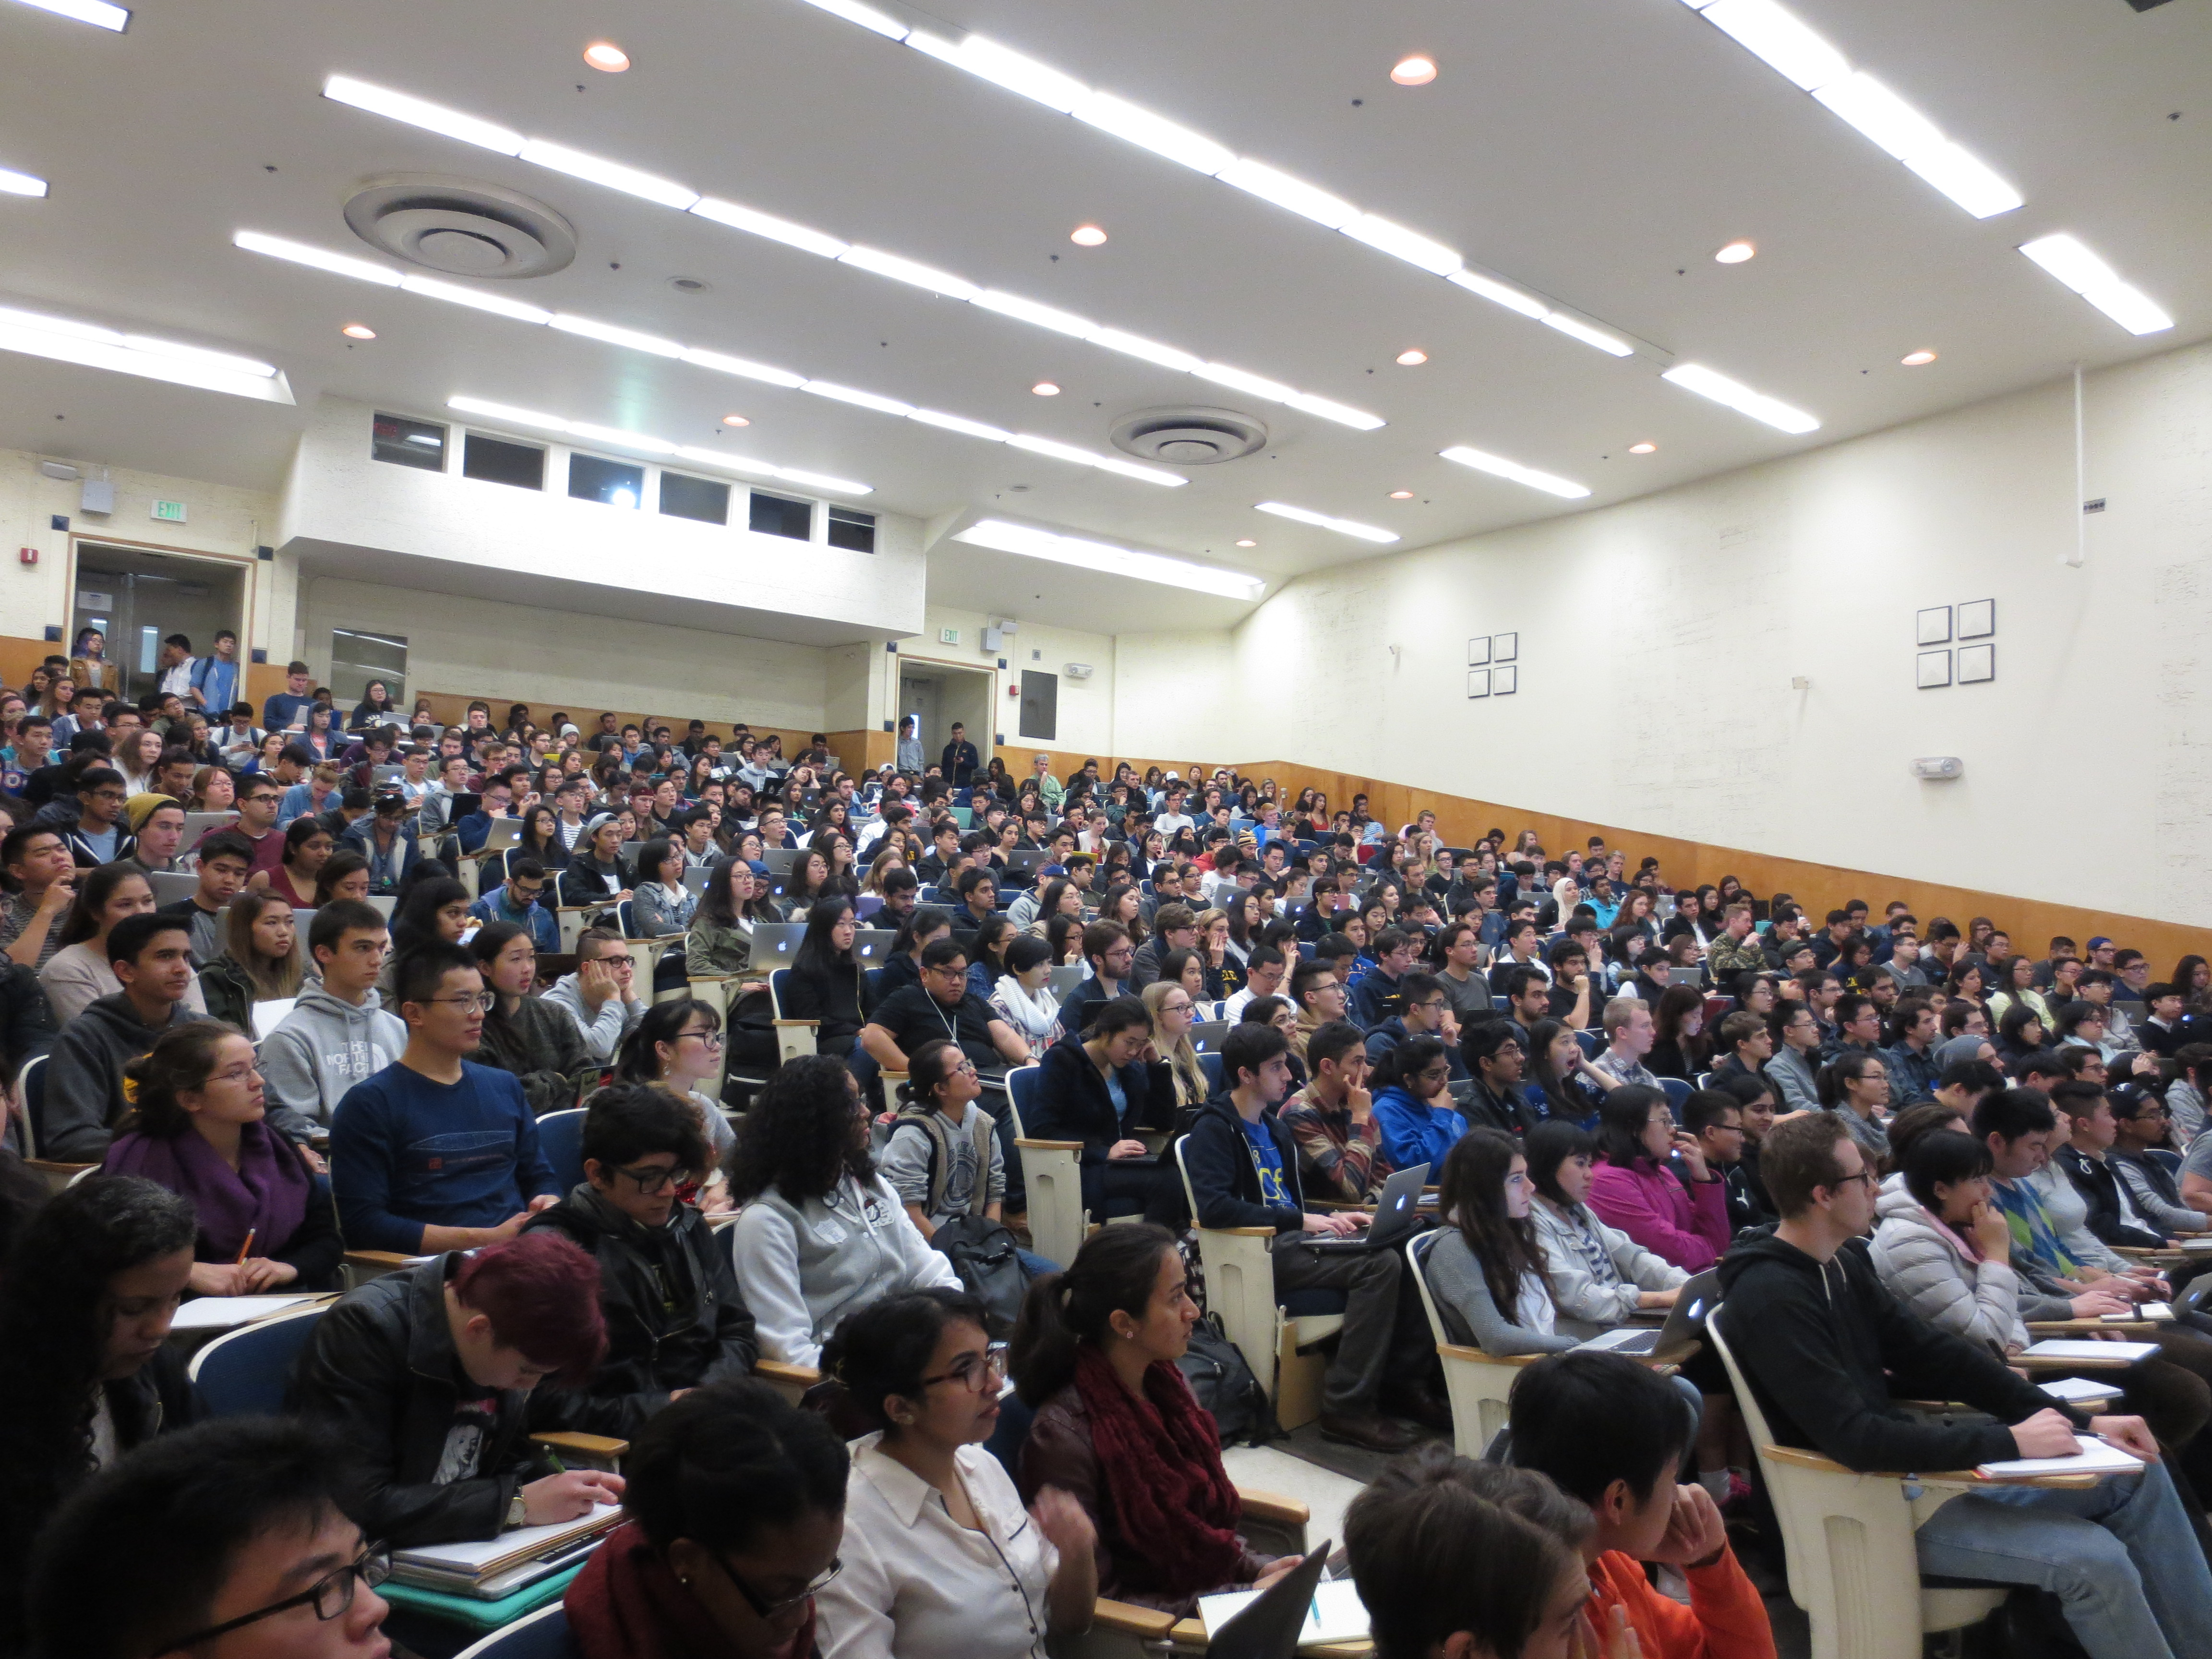
\includegraphics[width=0.9\textwidth]{fig/DS8.jpg} \\
Data Science 8, Spring 2016 at UC Berkeley
\end{center}
}

\frame{
\todo{flesh out intro!!}
}

\section[Examples]{Examples}
\subsection[Teaching evaluations]{Gender bias in teaching evaluations}


\frame
{
  \frametitle{Teaching Evaluations}
 \begin{center}
 \Large{ Student evaluations of teachers (SET) are used to} \\
  \begin{itemize}
  \item Quantify teaching effectiveness
  \item Compare instructors across courses
  \item Make hiring, firing, and promotion decisions  
  \end{itemize}
  \vfill
Are SET a valid measure of teaching effectiveness? 
\end{center}
}


\frame{
\frametitle{Teaching evaluations}
\large

In \citet{boring2016teaching}, we reanalyzed data from \cite{macnell2014whats}.
\vspace{10pt}
\begin{center}
\begin{itemize}
\itemsep 10pt
\item Students were randomized to 4 online sections of a course.
\item In two sections, the instructors swapped identities.
%\item Female-identified instructor was rated lower on average in all categories
\item Was the instructor who identified as female rated lower on average?
\end{itemize}
\end{center}
}


\frame{
\frametitle{Neyman-Rubin model, generalized}
Student $i$ is represented by a ticket with $4$ numbers, their response to each ``treatment.''

\begin{align*}
r_{ijk} &= \text{ SET given by student }i\text{ to instructor }j \\
&\text{ when they appear to have gender }k
\end{align*}
$$i = 1, \dots, N; \qquad j = 1,2; \qquad k \in \{ \text{male, female} \}$$

\vspace{10pt}
Numbers are fixed; randomization reveals one of the numbers. \\
\vspace{10pt}
Assume non-interference: each student's response depends only on that student's treatment. \\
\vspace{10pt}
If gender doesn't matter,
$$r_{ij\text{male}} = r_{ij\text{female}}.$$
}


\frame{
\frametitle{Randomization}

Conceptually, there are two levels of randomization:

\begin{enumerate}
\item $N_m$ students are randomly assigned to the male instructor, and
the remaining $N_f$ get the female instructor.
\item Of the $N_j$ assigned to instructor $j$, 
$N_{jm}$ are told that the instructor is male, for $j = 1, 2$.
\end{enumerate}
\vspace{10pt}

All ${{N_m}\choose{N_{mm}} }\times{ {N_f}\choose{N_{fm}}}$ assignments of students to sections
are equally likely. \\
\vspace{10pt}

\begin{block}{Stratified two-sample test}
\begin{itemize}
\item For each instructor, permute perceived gender assignments
\item Use difference in mean ratings for female-identified minus male-identified
\end{itemize}
\end{block}
}

\begin{frame}[fragile]
\frametitle{Code}
\begin{center}
\begin{rcode}
# Load data
library(permuter)
data(macnell)


# Calculate the observed test statistic
tst_stat <- function(x) {
  mean(x[macnell$taidgender == 0], na.rm = TRUE) -
  mean(x[macnell$taidgender == 1], na.rm = TRUE)
  }
observed <- tst_stat(macnell$overall)

# Ratings vs reported instructor gender (difference in means)
distr <- stratified_two_sample(response=macnell$overall, 
                               group=macnell$taidgender, 
                               stratum=macnell$tagender,
                               stat="mean", reps=10**5)


# Calculate two-sided p-value
p <- t2p(observed, distr, alternative = "two-sided")

\end{rcode}
\end{center}
\end{frame}


\frame
{
  \frametitle{Results}
In all categories, the male-identified instructor was rated higher.
\begin{table}
\begin{tabular}{r|crr}
\textbf{Characteristic} & \textbf{M-F} & \textbf{perm} $P$ & \textbf{t-test} $P$ \\
\hline
Overall & 0.47 & 0.12 & 0.128\\
Caring & 0.52 & 0.10 & 0.071\\
Consistent & 0.47 & 0.21 & \textcolor{red}{0.045} \\ 
Enthusiastic & 0.57 & 0.06 & 0.112 \\
Fair & 0.76 & \textcolor{red}{0.01} & 0.188 \\
Feedback & 0.47 & 0.16 & 0.054 \\
Helpful & 0.46 & 0.17 & \textcolor{red}{0.049} \\
Knowledgeable & 0.35 & 0.29 & \textcolor{red}{0.038} \\
Praise & 0.67 & \textcolor{red}{0.01} & 0.153 \\
Professional & 0.61 & 0.07 & 0.124 \\
Prompt & 0.80 & \textcolor{red}{0.01} & 0.191 \\
Respectful & 0.61 & 0.06 & 0.124 \\
Responsive & 0.22 & 0.48 & \textcolor{red}{0.013}
\end{tabular}
\end{table}

}



\frame{
\frametitle{Omnibus Test}
\textbf{Nonparametric combination of tests (NPC):} combine individual p-values into a single omnibus test when there are many responses \\
\vspace{10pt}

Test whether to accept \textbf{all null} hypotheses or reject \textbf{at least one alternative} \\
\vspace{10pt}

\begin{block}{Fisher's combining function}
Let $\{ P_j\}_{j=1}^J$ be p-values for $J$ hypotheses. Define
$$X^2 = -2 \sum_{j=1}^J \ln(P_j)$$
If $\{ P_j\}_{j=1}^J$ are independent and all nulls are true, then $X^2 \sim \chi_{2J}^2$ . \\
\end{block}
}


\frame{
\frametitle{Omnibus Test}
Ratings by the same student for different categories are \textbf{dependent}.\\
\vspace{10pt}

$\implies$ Treat all ratings from a student as a vector and calibrate the distribution of $X^2$ using the this permutation distribution.
\vspace{10pt}

\begin{block}{NPC Permutation Procedure}
\begin{enumerate}
\item Calculate the vector of test statistics (use the \textbf{same permutation} of section memberships to compute all statistics), repeat a large number $B$ times
\item Compute the p-value for each individual variable in each permutation relative to the other values in the distribution
\item Apply the combining function to each vector of p-values.
\end{enumerate}
\end{block}
}



\begin{frame}[fragile]
\frametitle{Omnibus Test}
\begin{rcode}
# Initialize placeholders
categories <- colnames(macnell)[2:16]
test_distr <- matrix(0, nrow = 10**5, ncol = length(categories))
pvalues <- rep(0, length(categories))
colnames(test_distr) <- names(pvalues) <- categories

# Loop over rating categories
for(col in categories){
  set.seed(678)
  observed <- tst_stat(macnell[ ,col])
  distr <- stratified_two_sample(response=macnell[ ,col], 
                                 group=macnell$taidgender, 
                                 stratum=macnell$tagender,
                                 stat="mean", reps=10**5)
  test_distr[, col] <- distr
  pvalues[col] <- t2p(observed, distr, alternative = "two-sided")
}

# NPC 
omnibus_pvalue <- npc(pvalues, test_distr, combine="fisher", 
                     alternatives="two-sided")

\end{rcode}
\end{frame}

\frame{
\frametitle{Conclusions}
\large
\textbf{Omnibus test:} $P = 0$ \\
\vspace{20pt}

Reject the null hypothesis that there is no difference in ratings for any category. \\
\vspace{10pt}
$\implies$ SET measure something other than teaching effectiveness.
}


\subsection[Inter-rater reliability]{Inter-rater reliability}
\frame{
\frametitle{Inter-rater reliability test}
\large
\begin{itemize}
\itemsep10pt
\item Naomi Stark and Gilbert Kliman (NSGK) collected videos of therapy sessions with children on the autism spectrum
\item A team of trained raters watched and tagged each 30-second interval of video from a collection of 183 clinically relevant tags
\item Is tagging of therapist-patient interactions reliable (\cite{millman2016case})? 
\end{itemize}
}

\frame{
\frametitle{Inter-rater reliability test}
There are four dimensions. Can we simplify?
\vspace{10pt}
\begin{itemize}
\item Consider each clinical tag individually
\item Do a partial hypothesis test for each video, then combine using NPC
\end{itemize}
\vspace{10pt}
%}
%
%\frame{
%\frametitle{Inter-rater reliability test}
\begin{table}[h]
\begin{center}
\begin{tabular}{ | c | c | }
  \hline
  \textbf{NSGK} & \textbf{IRR}  \\
  \hline
  183 types of activity  & $T$ tags  \\
  \hline
  8 videos  & $S$ strata   \\
  \hline
  $\sim$35 segments/video  & $N_s$ items/stratum   \\
  \hline
  10 raters  & $R$ raters  \\
  \hline
\end{tabular}
\end{center}
\end{table}
}

\frame{
\frametitle{Inter-rater reliability test}
We need
\begin{itemize}
\item a test statistic for concordance
\item a chance model
\end{itemize}

\begin{figure}
\centering
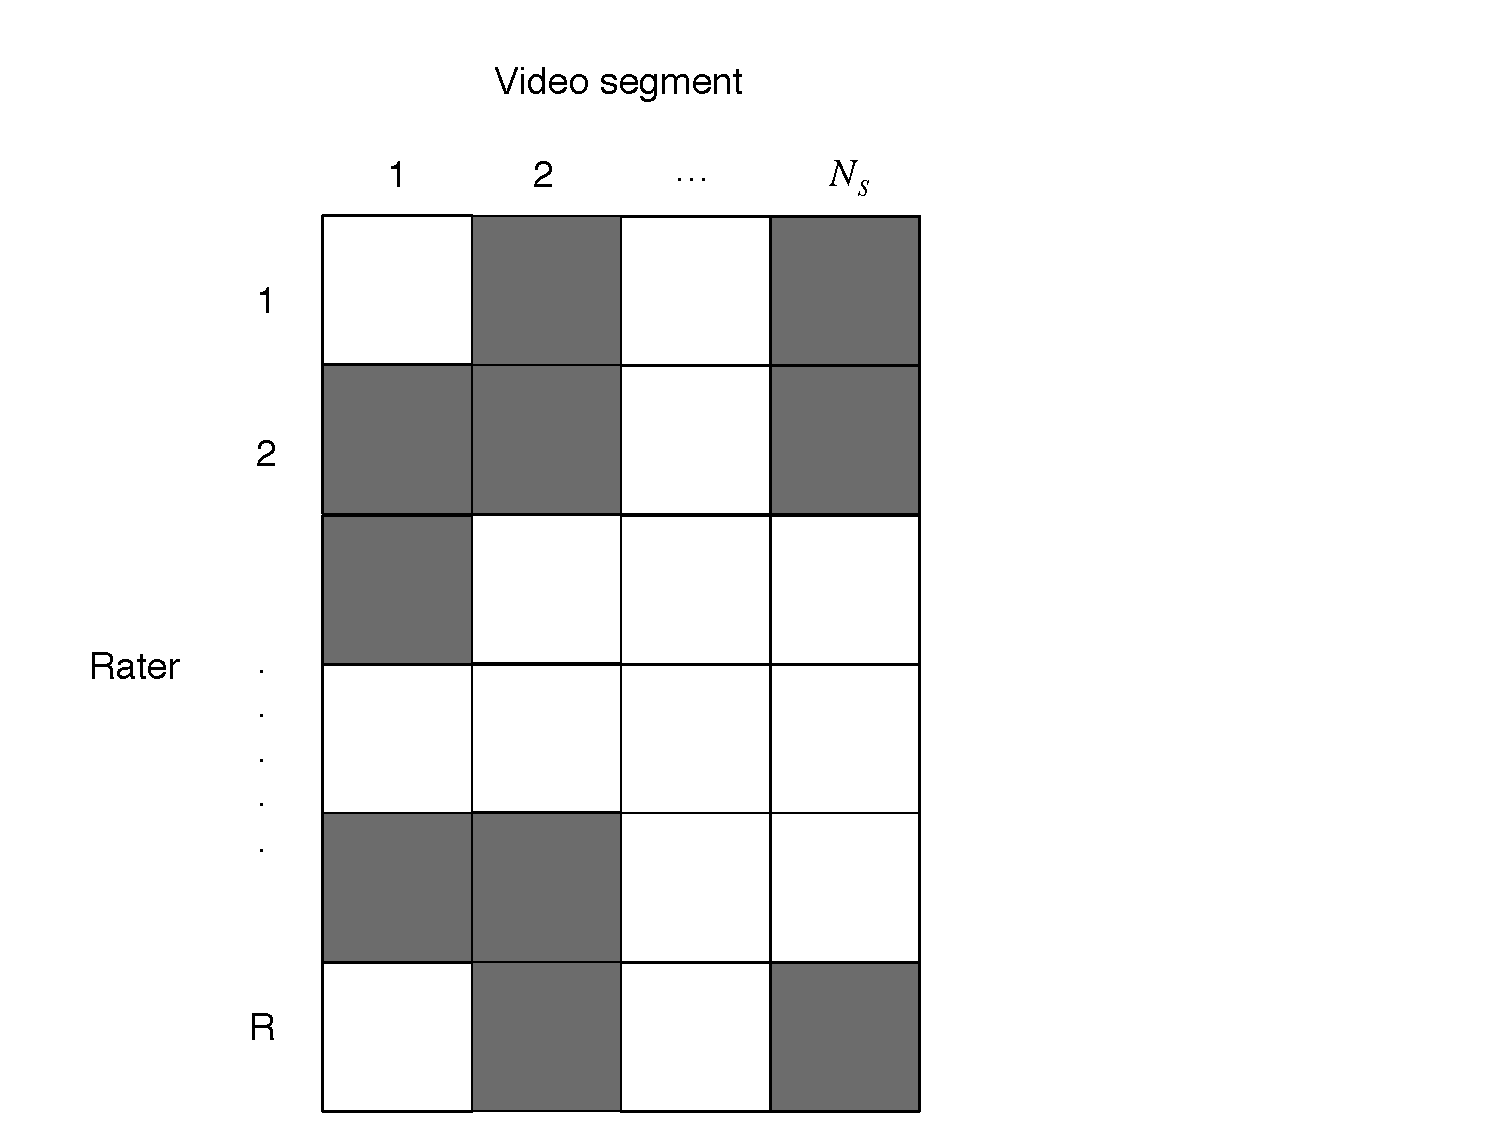
\includegraphics[height=0.65\textheight]{fig/irr/perm1}
\end{figure}
}


\frame{
\frametitle{Inter-rater reliability test}
Define
\begin{itemize}
\item $\{ L_{s,i,r} \} = $ indicator for whether rater $r$ tagged item $i$ in stratum $s$
\item $y_{si} = \sum_{r=1}^R L_{s,i,r} =$ number of raters who tagged item $i$ in stratum $s$
\end{itemize}

\vspace{10pt}
The test statistic within stratum $s$ is

\begin{align*}
\rho_s &\equiv \frac{1}{N_s {R \choose 2}} \sum_{i=1}^{N_s}
              \sum_{r=1}^{R-1} \sum_{v=r+1}^R \mathbf{1}(L_{s,i,r} = L_{s,i,v}) \\
              &= \frac{1}{N_s R(R-1)} \sum_{i=1}^{N_s}
                (y_{si}(y_{si}-1) + (R-y_{si})(R-y_{si}-1)).
\end{align*}

}

%
%\frame{
%\frametitle{Inter-rater reliability test}
%Now we have a measure of concordance. 
%\begin{figure}
%\centering
%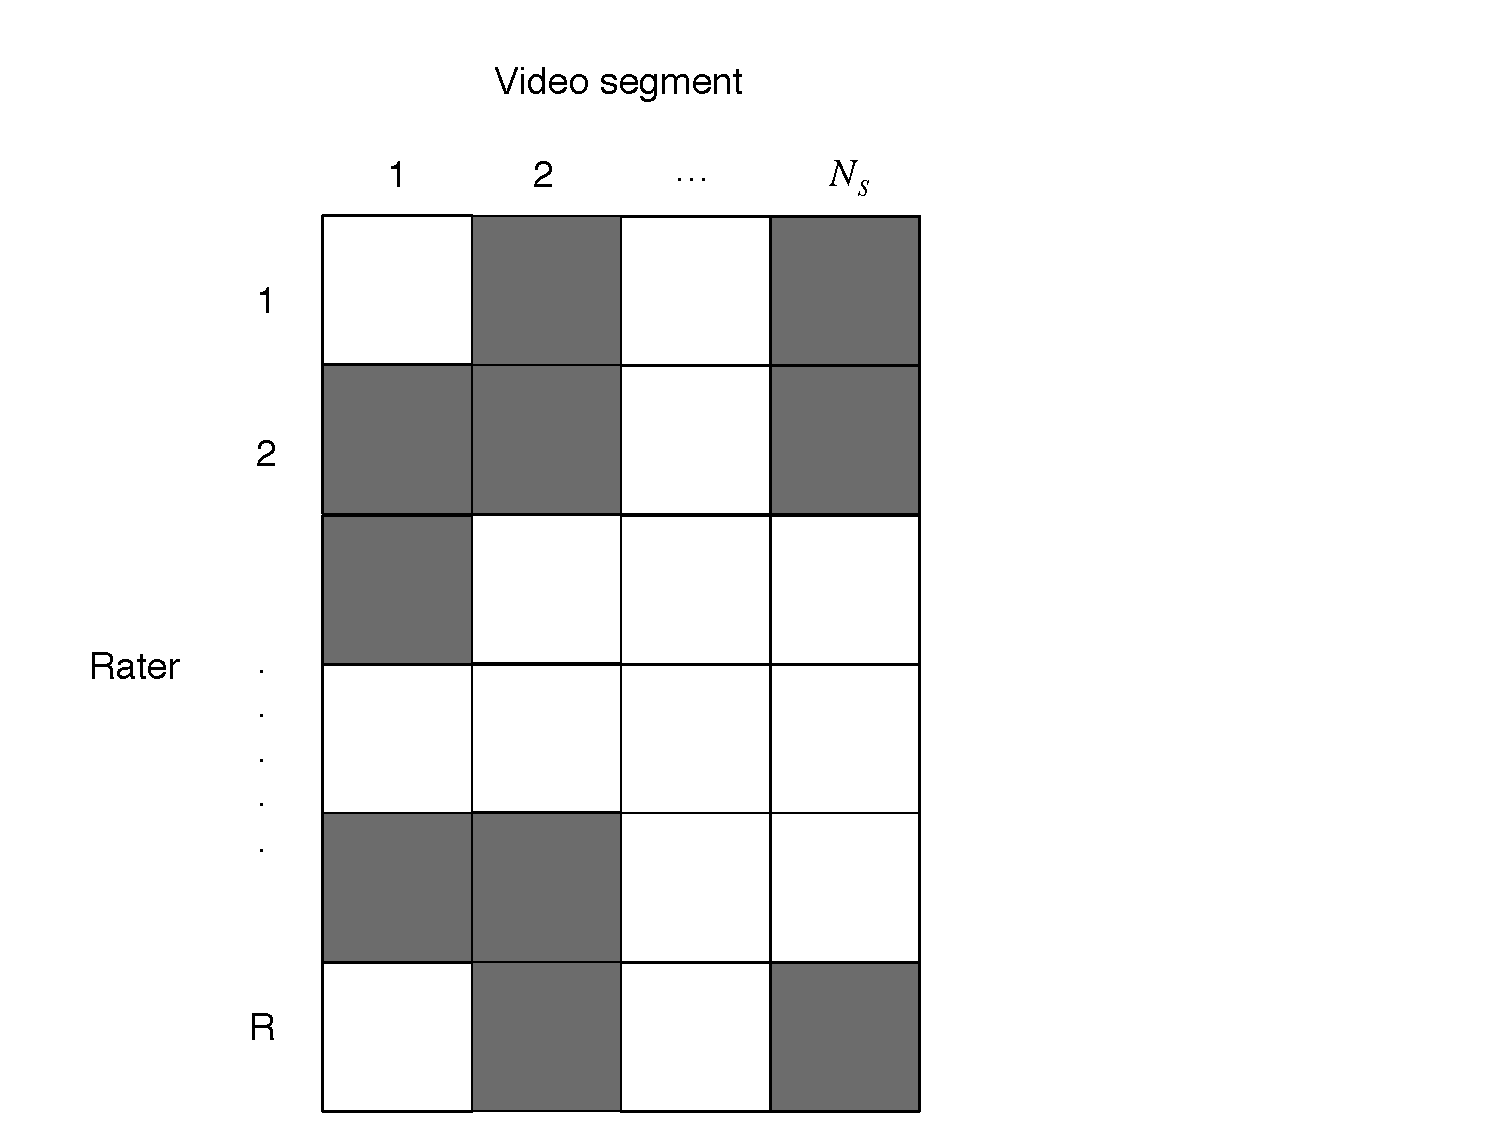
\includegraphics[height=0.75\textheight]{fig/irr/perm1}
%\end{figure}
%}

\frame{
\frametitle{Permutation test}
If tags are assigned completely at random, conditional on the number of items each rater tagged, then

\begin{itemize}
\item all possible permutations of tags are likely for an individual rater
\item raters assign tags independently of each other
%\item \textbf{Implied randomization:} Permute tags within rows, independently across rows and across strata.
\end{itemize}


\begin{block}{IRR Permutation Test}
\begin{itemize}
\item Compute $\rho_s$ for $s = 1, \dots, S$ for the observed data
\item Permute tags within rows, independently across rows and across strata, to get the permutation distributions
\item For the observed and permutation $\rho_s$ values, find the corresponding p-value $P_s$ for each permutation
\item The NPC test statistic is $T = -\sum_{s=1}^S \frac{P_s}{\sqrt{N_s}}$.
\end{itemize}
\end{block}
}

%\frame{
%\frametitle{Inter-rater reliability test}
%Observed tags for stratum $s$
%\begin{figure}
%\centering
%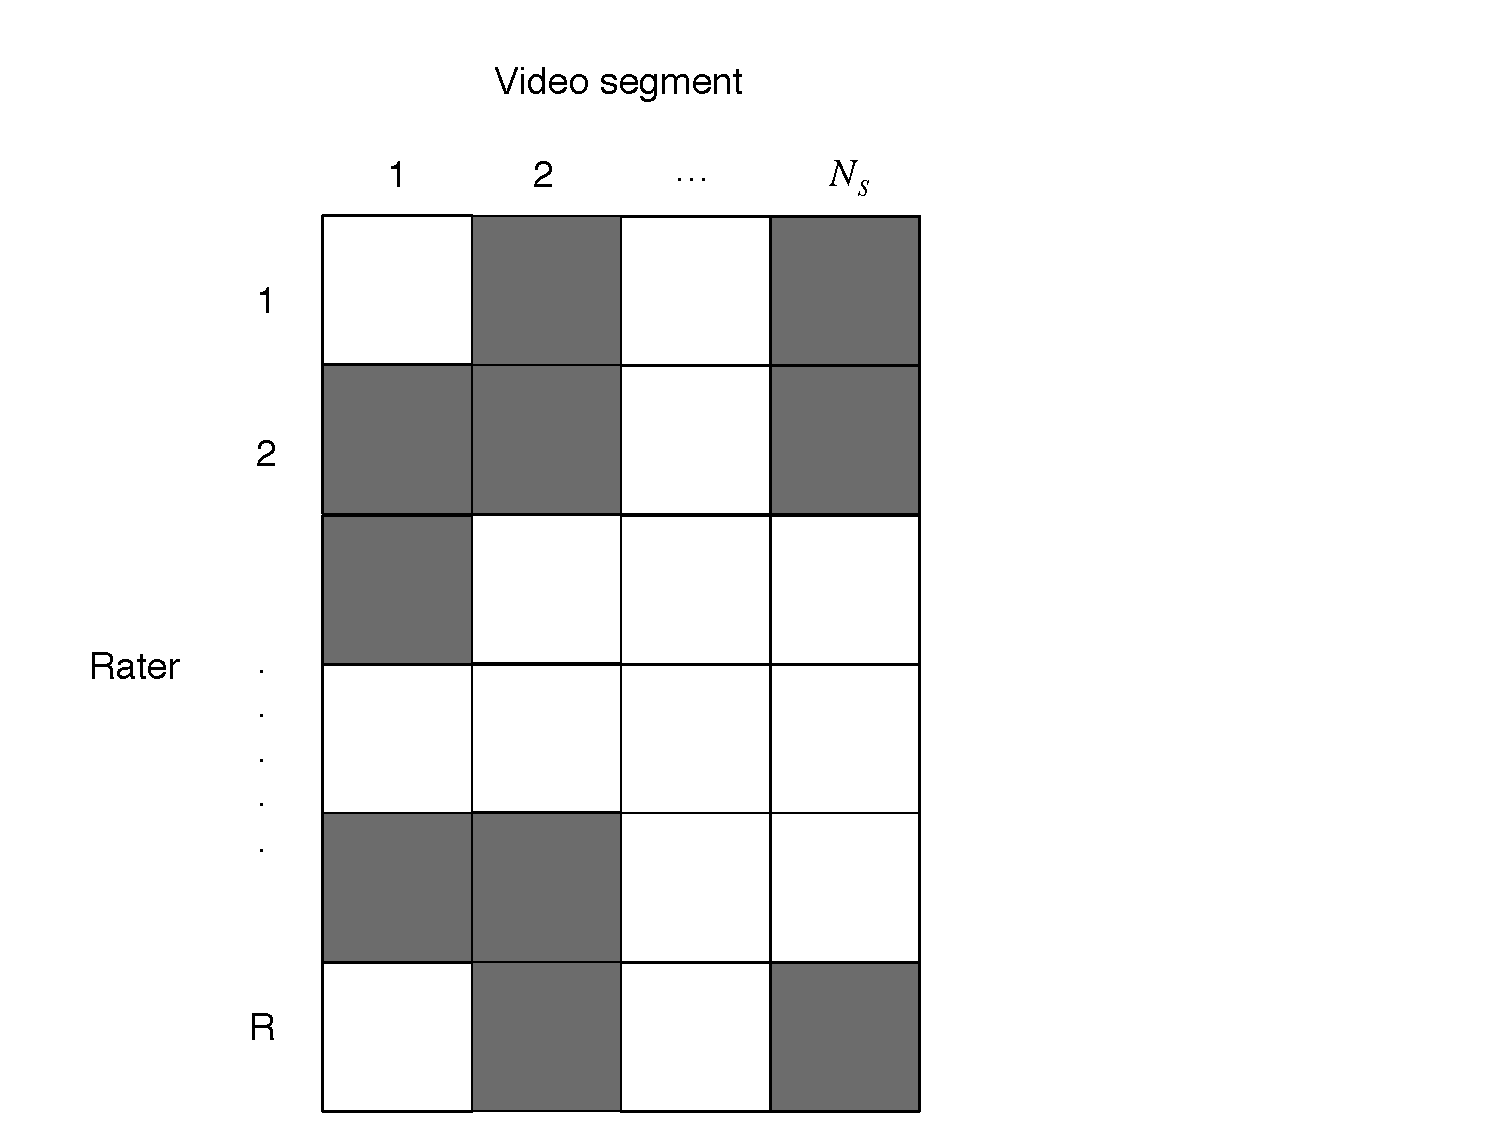
\includegraphics[height=0.75\textheight]{fig/irr/perm1}
%\end{figure}
%}\frame{
%\frametitle{Inter-rater reliability test}
%Equally likely tags for stratum $s$, under the null
%\begin{figure}
%\centering
%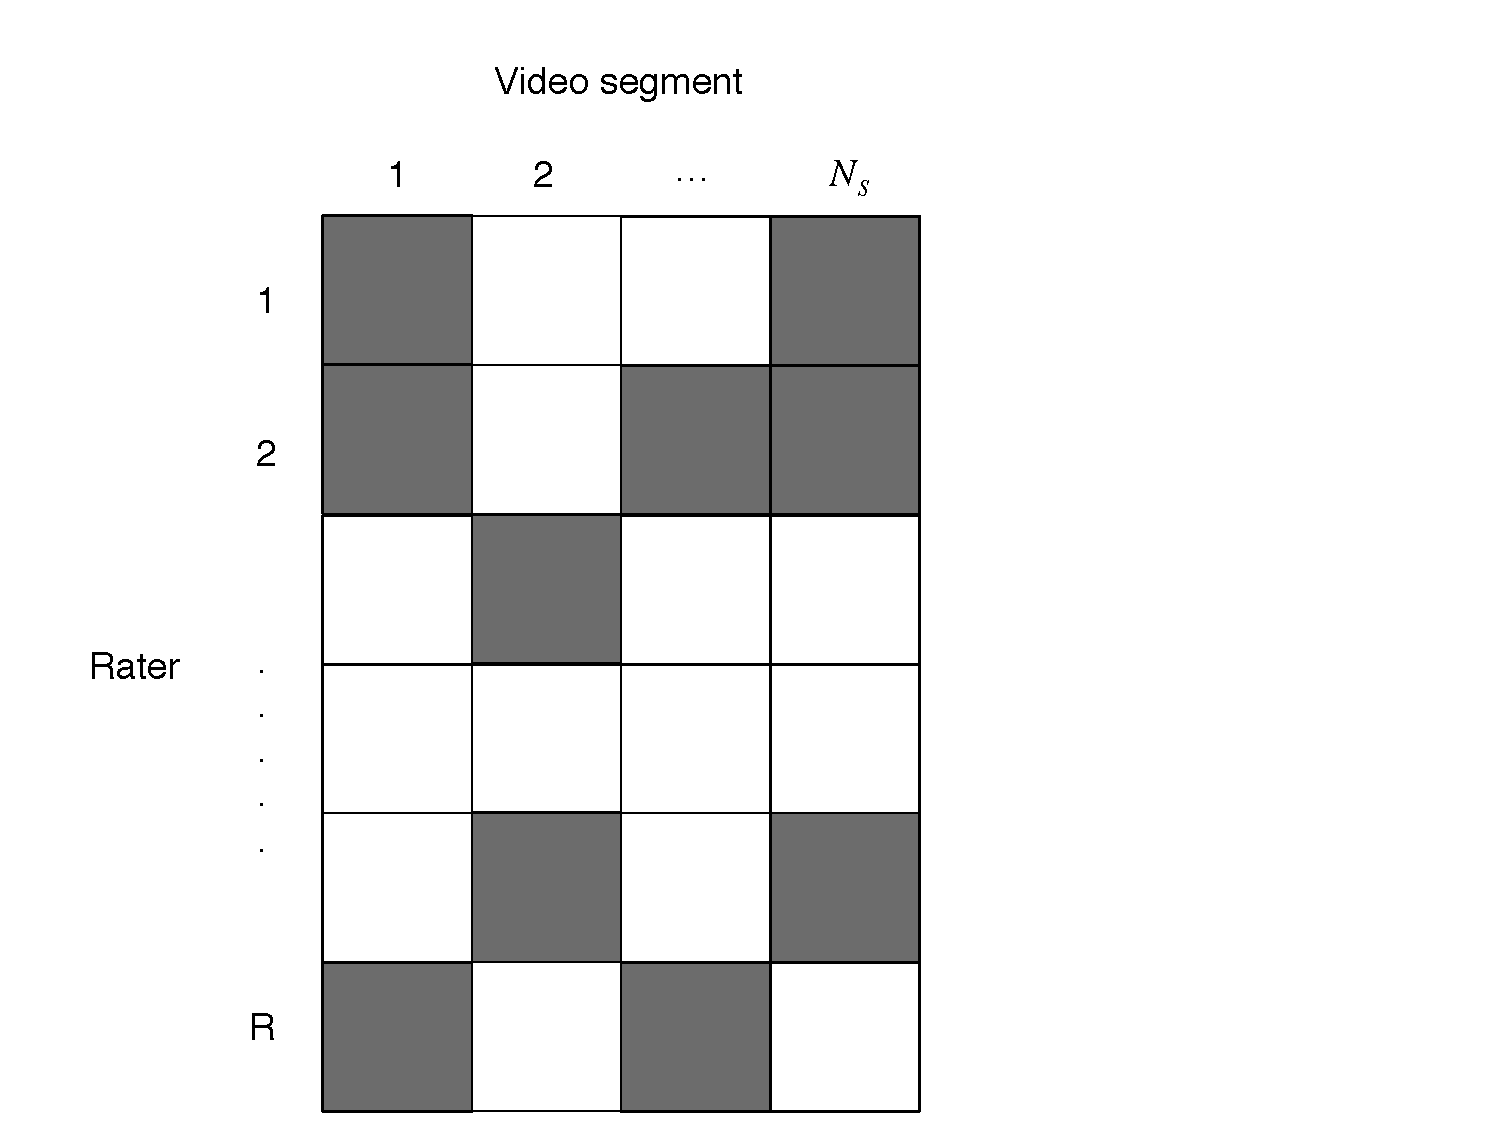
\includegraphics[height=0.75\textheight]{fig/irr/perm2}
%\end{figure}
%}
%\frame{
%\frametitle{Inter-rater reliability test}
%Equally likely tags for stratum $s$, under the null
%\begin{figure}
%\centering
%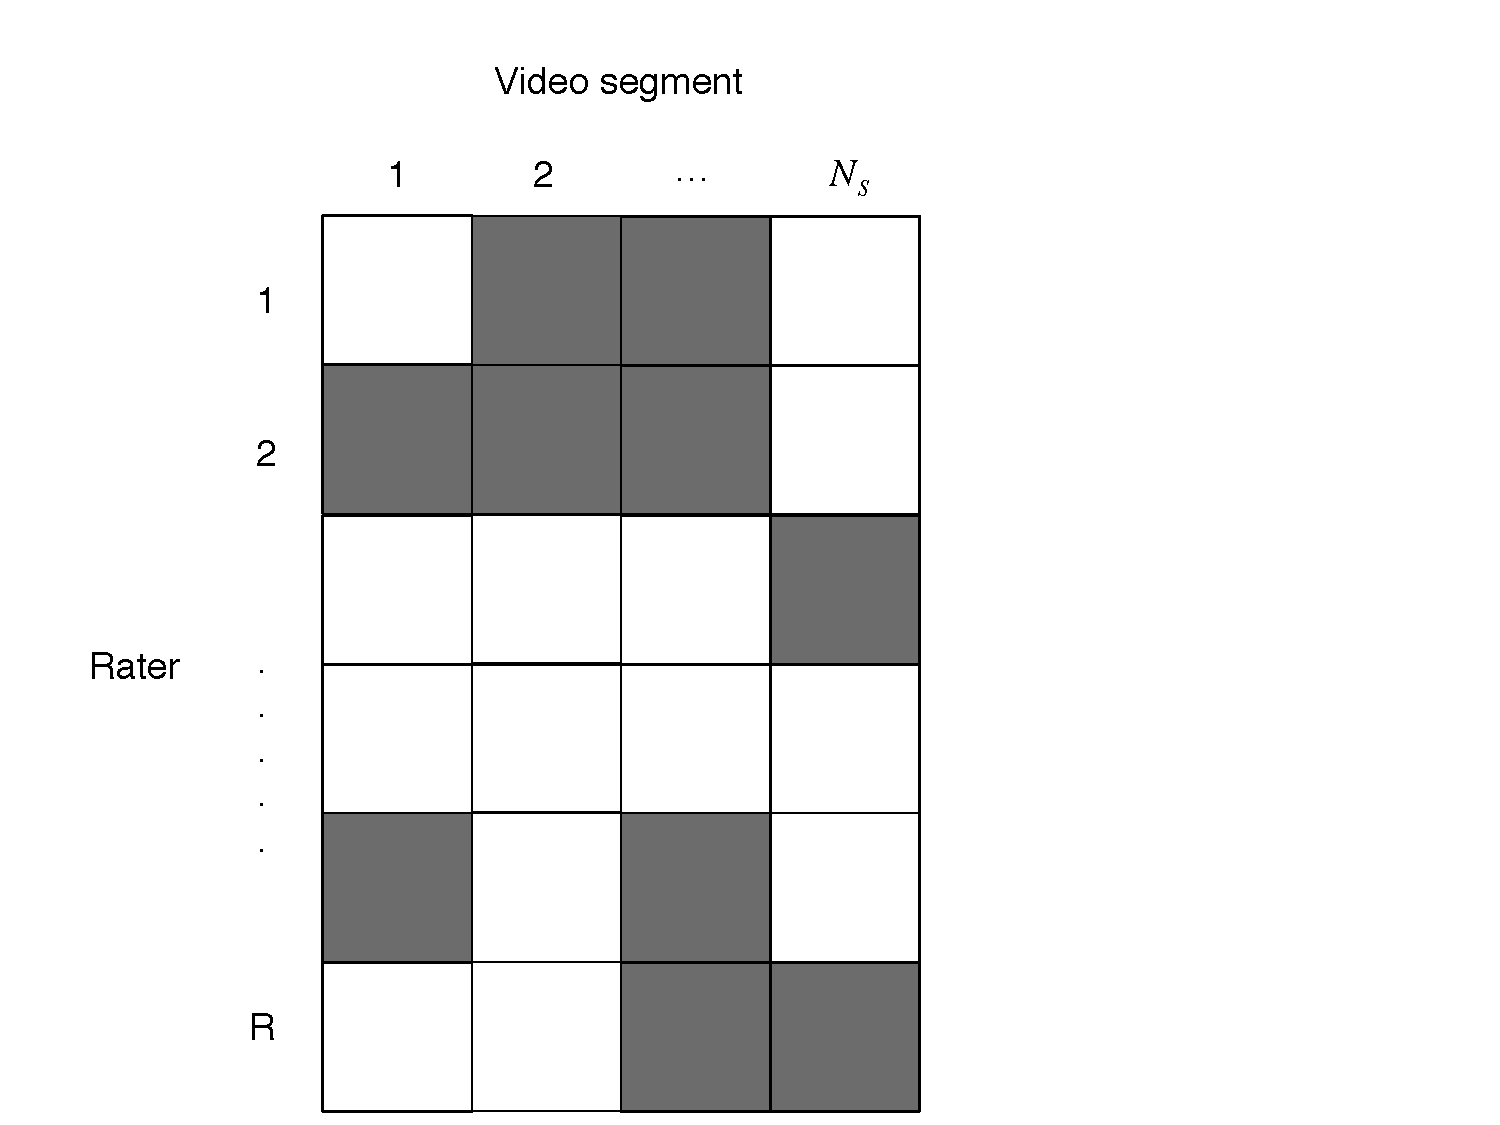
\includegraphics[height=0.75\textheight]{fig/irr/perm3}
%\end{figure}
%}



\begin{frame}[fragile]
\frametitle{Code}
\begin{rcode}
# NSGK example

library(permuter)
library(dplyr)
library(ggplot2)

data(nsgk)
time_stamps <- c(36, 32, 35, 37, 31, 35, 40, 32)

# nsgk_mat is a list of lists:
# first level indexes the tag
# second level indexes the video
# For how to obtain nsgk_mat from data(nsgk), see the vignette nsgk.Rmd


# Example of how we analyze a single tag.
tag1 <- nsgk_mat[[1]]

# Find the distribution of the IRR test statistic for each video
video_specific_results <- lapply(tag1, function(x){
  res <- irr_ts_distribution(x, num_perm = 1000,    
                            keep_dist = TRUE, seed = 101)
})
tag_distribution <- sapply(video_specific_results, function(x) x$dist)
tag_pvalues      <- sapply(video_specific_results, function(x) x$pvalue)

# Combine across videos with NPC
tag_npc_res <- irr_npc_distribution(tag_distribution, size = time_stamps, pvalues = tag_pvalues)

\end{rcode}

\end{frame}

\frame{
\frametitle{Results}

\todo{\begin{itemize}
%\item 50 tags were never used
\item 60 tags had $P < 0.05$
\item Statistical vs practical significance -- consult domain scientists 
\item Is there a more useful summary statistic than $\rho_s$?
\end{itemize}
}
\begin{figure}[htbp]
\begin{center}
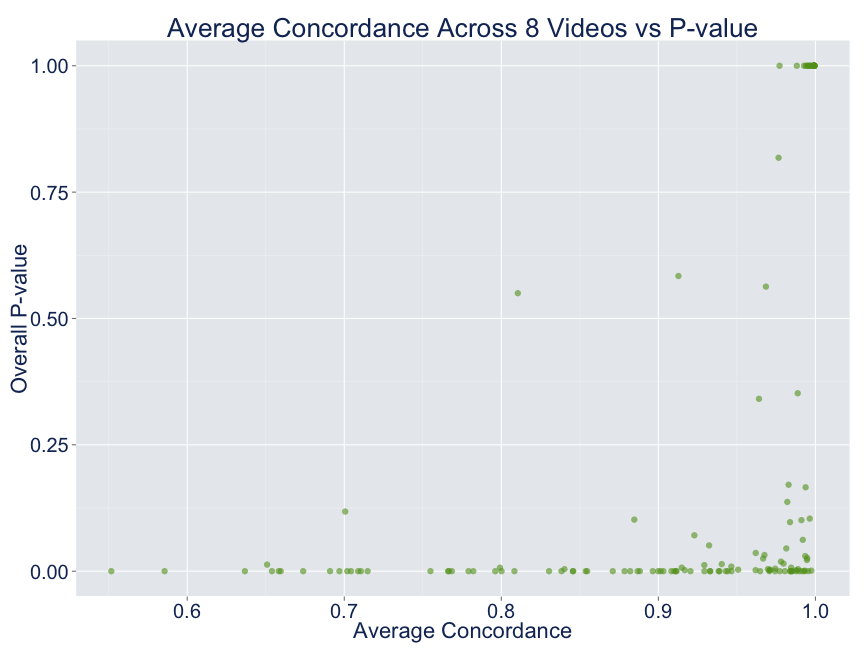
\includegraphics[height=0.7\textheight]{fig/nsgk}
\end{center}
\end{figure}

}



\section[Software and Statistics]{The role of software development in Statistics}

\frame{
\frametitle{Software and Statistics}
\Large
Why should Statisticians worry about writing software?

\begin{itemize}
\item Ethics
\item Impact
\end{itemize}
}


\frame{
\frametitle{Ethics}

\includegraphics[width=\textwidth]{fig/repro.png}
}

%\frame{
%\frametitle{Ethics}
%\textbf{Much of the reproducibility crisis can be traced back to bad statistics.} 
%
%\begin{itemize}
%\item Publication bias: positive findings are more likely to get published
%\item P-hacking and the garden of forking paths (\cite{gelman2013garden})
%\item Inappropriate statistical tests (Randomization inference may help here)
%\end{itemize}
%\vspace{15pt}
%\large We must make it easy for researchers to do the right statistics.
%}

\frame{
\frametitle{Impact}
\large

\begin{block}{Bin~\cite{yu2014datascience}}
Let us own data science.
\end{block}


\vspace{20pt}
\textbf{Statisticians} have to build the tools to
\begin{itemize}
\itemsep5pt
\item facilitate reproducible scientific research,
\item enable people to use the methods we develop (correctly!), and
\item impact the way people think about data.
\end{itemize}
}

\frame{
\frametitle{Download \texttt{permute}!}
\begin{figure}[htbp]
\begin{center}
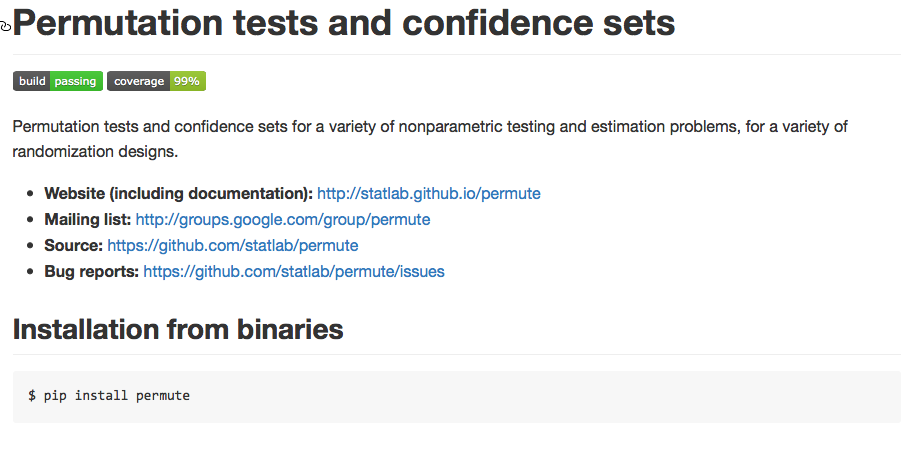
\includegraphics[width=\textwidth]{fig/github/permute}
\end{center}
\end{figure}


\url{https://github.com/statlab/permute}
}


\begin{frame}
\frametitle{References}
\tiny
\bibliographystyle{plainnat}
\bibliography{refs}
\itemize
\end{frame}


\end{document}